% =============================================================
%  Data Center Availability — Methodology & Topology Comparison
%  Adapted from the standalone deck into the American Terawatt template.
%  (Tier III vs. Tier IV; RBD availability methodology.)
% =============================================================

%---- Local palette & RBD node styles (used by the TikZ diagrams) ----
\definecolor{accent}{HTML}{1F6FB2}   % blue  = redundant / result
\definecolor{surf}{HTML}{F2F4F7}     % light surface
\definecolor{surf2}{HTML}{E1ECF4}    % accent surface
\definecolor{edge}{HTML}{8A94A6}     % connectors

\tikzset{
  box/.style   ={draw=edge, rounded corners=3pt, minimum width=2.1cm,
                 minimum height=0.85cm, align=center, font=\scriptsize,
                 fill=surf, thick},
  redbox/.style={box, draw=accent, double, double distance=1.3pt, line width=0.7pt},
  load/.style  ={draw=accent, line width=1.4pt, rounded corners=3pt,
                 minimum width=2.0cm, minimum height=1.0cm, align=center,
                 font=\scriptsize\bfseries, fill=surf2},
  cont/.style  ={box, minimum width=6.2cm, minimum height=0.95cm},
  redcont/.style={cont, draw=accent, double, double distance=1.3pt, line width=0.7pt},
  flow/.style  ={-{Latex[length=2mm]}, edge, thick},
  tag/.style   ={font=\tiny\bfseries, text=accent},
  andgate/.style={draw=edge, circle, fill=surf, thick, inner sep=1pt,
                  minimum size=0.95cm, font=\tiny\bfseries, text=edge, align=center},
}

% \sectionslide{Data Center Availability}{Calculation methodology \& topology comparison (Tier III vs.\ Tier IV)}

% ============================================================
\intermezzo{Data Center Availability}{Calculation methodology \& topology comparison}

\begin{frame}{Abbreviations}
  \centering
  \renewcommand{\arraystretch}{1.3}
  \begin{tabular}{ll}
    \toprule
    \textbf{CRAH} & Computer Room Air Handler \\
    \textbf{FMEA} & Failure Mode and Effects Analysis \\
    \textbf{MTBF} & Mean Time Between Failures \\
    \textbf{MTTR} & Mean Time To Repair \\
    \textbf{MV / LV} & Medium / Low Voltage \\
    \textbf{PDU}  & Power Distribution Unit \\
    \textbf{RBD}  & Reliability Block Diagram \\
    \textbf{TIA}  & Telecommunications Industry Association (TIA-942) \\
    \textbf{UPS}  & Uninterruptible Power Supply \\
    \bottomrule
  \end{tabular}
\end{frame}



\begin{frame}{What ``availability'' means}
  Availability is the fraction of time a facility (or system) can deliver IT load
  without interruption, measured over a defined period (typically a rolling 12 months).

  \vspace{0.6em}
  \begin{block}{Core relationship}
    \[
      A \;=\; \frac{\text{Uptime}}{\text{Uptime}+\text{Downtime}}
        \;=\; \frac{\mathrm{MTBF}}{\mathrm{MTBF}+\mathrm{MTTR}}
    \]
  \end{block}
  \vspace{0.3em}
  where\\ 
  \quad\textbf{MTBF} is mean time between failures\\
  \quad\textbf{MTTR} is mean time to repair/recover.\\
  \vspace{1em}
  Availability is reported as a percentage or in ``nines.''
\end{frame}

\begin{frame}{The language of nines}
  \centering
  \renewcommand{\arraystretch}{1.25}
  \begin{tabular}{lcc}
    \toprule
    \textbf{Availability} & \textbf{Nines} & \textbf{Allowable downtime / yr} \\
    \midrule
    99\,\%      & two   & $\approx$ 3.65 days   \\
    99.9\,\%    & three & $\approx$ 8.77 hours  \\
    99.99\,\%   & four  & $\approx$ 52.6 minutes\\
    99.999\,\%  & five  & $\approx$ 5.26 minutes\\
    99.9999\,\% & six   & $\approx$ 31.5 seconds\\
    \bottomrule
  \end{tabular}

  \vspace{1em}
  \small Every additional nine cuts allowable downtime by a factor of ten.
\end{frame}

\begin{frame}{Combining components}
  A facility is modeled as a reliability block diagram (RBD) of components in
  \emph{series} and \emph{parallel}.

  \vspace{0.4em}
  \begin{columns}[T]
    \column{0.5\textwidth}
      \begin{block}{Series --- all required}
        \[ A = \prod_i A_i \]
        Any element fails $\Rightarrow$ outage.\\
        Always \emph{below} the weakest link.
      \end{block}
    \column{0.5\textwidth}
      \begin{block}{Parallel --- redundant}
        \[ A = 1 - \prod_i (1-A_i) \]
        Survives if $\geq 1$ path works.\\
        Redundancy raises $A$ sharply.
      \end{block}
  \end{columns}

  % \vspace{0.5em}
  % \begin{alertblock}{$N{+}1$ unit group (tolerates one failure)}
  %   \[ A_{\text{grp}} = A^{N+1} + (N{+}1)\,A^{N}(1-A) \]
  % \end{alertblock}
\end{frame}


\begin{frame}{Modeling assumptions}
  \textbf{Frameworks}
    \begin{itemize}
      \item Uptime Institute Tier standard (I--IV)
      \item TIA-942 infrastructure standard
      \item RBD, FMEA, Monte Carlo for complex topologies
    \end{itemize}
  \vspace{1em}
  \textbf{Scope}
    \begin{itemize}
      \item Facility \emph{infrastructure} availability
      \item Facility $=$ Power path $\times$ Cooling path
    \end{itemize}
\end{frame}


\begin{frame}{Reading the topology diagrams}
  \begin{columns}[T]
    \column{0.5\textwidth}
      \textbf{Redundancy notation}
      \begin{itemize}
        \item $N$ --- just enough capacity, no spare
        \item $N{+}1$ --- one spare unit
        \item $2N$ --- fully duplicated
      \end{itemize}
    \column{0.5\textwidth}
      \textbf{Border legend}
      \vspace{0.4em}

      \begin{itemize}
        \item \textcolor{accent}{\rule{0.55em}{0.55em}}\; \textbf{Double border} $=N{+}1$ redundant stage
        \item \textcolor{edge}{\rule{0.55em}{0.55em}}\; \textbf{Single border} $=$ single (concurrently maintainable) path
      \end{itemize}

      \vspace{0.8em}
      \centering
      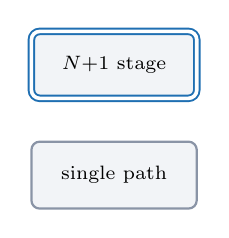
\begin{tikzpicture}
        \node[redbox] (r) at (0,1.4) {$N{+}1$ stage};
        \node[box]    (s) at (0,0)   {single path};
      \end{tikzpicture}
  \end{columns}
\end{frame}

\begin{frame}{Tier I topology}
  \centering
  \resizebox{0.94\textwidth}{!}{%
  \begin{tikzpicture}
    \node[box] (S) at (0,1.7)  {Source\\{\tiny Utility $\parallel$ Gen}};
    \node[box] (U) at (2.7,1.7){UPS\\{\tiny 1 module ($N$)}};
    \node[box] (D) at (5.4,1.7){Distribution\\{\tiny single path}};
    \node[box] (C) at (0,0)   {Chiller\\{\tiny 1 unit ($N$)}};
    \node[box] (P) at (2.7,0) {Pump\\{\tiny 1 unit ($N$)}};
    \node[box] (R) at (5.4,0) {CRAH\\{\tiny 1 unit ($N$)}};
    \node[load] (L) at (8.9,0.85){IT Load\\{\tiny 99.671\%}};
    \node[andgate] (A) at (7,0.85) {AND};
    \draw[flow] (S) -- (U);   \draw[flow] (U) -- (D);
    \draw[flow] (C) -- (P);   \draw[flow] (P) -- (R);
    \draw[flow] (D.east) -| (A.north);
    \draw[flow] (R.east) -| (A.south);
    \draw[flow] (A.east) -- (L.west);
    \node[tag, anchor=west] at (-2.3,1.7) {POWER};
    \node[tag, anchor=west] at (-2.3,0)   {COOL};
  \end{tikzpicture}}

  \vspace{0.5em}
  {\footnotesize 
    \begin{itemize}
      \item No redundancy anywhere
      \item Single distribution path
      \item \emph{Not} concurrently maintainable - planned maintenance requires a shutdown
    \end{itemize}
  }
\end{frame}

\begin{frame}{Tier II topology}
  \centering
  \resizebox{0.94\textwidth}{!}{%
  \begin{tikzpicture}
    \node[box] (S) at (0,1.7)  {Source\\{\tiny Utility $\parallel$ Gen}};
    \node[redbox] (U) at (2.7,1.7){UPS\\{\tiny 1 module ($N$)}};
    \node[box] (D) at (5.4,1.7){Distribution\\{\tiny single path}};
    \node[redbox] (C) at (0,0)   {Chillers\\{\tiny 1 unit ($N$)}};
    \node[redbox] (P) at (2.7,0) {Pumps\\{\tiny 1 unit ($N$)}};
    \node[redbox] (R) at (5.4,0) {CRAH\\{\tiny 1 unit ($N$)}};
    \node[load] (L) at (8.9,0.85){IT Load\\{\tiny 99.741\%}};
    \node[andgate] (A) at (7,0.85) {AND};
    \draw[flow] (S) -- (U);   \draw[flow] (U) -- (D);
    \draw[flow] (C) -- (P);   \draw[flow] (P) -- (R);
    \draw[flow] (D.east) -| (A.north);
    \draw[flow] (R.east) -| (A.south);
    \draw[flow] (A.east) -- (L.west);
    \node[tag, anchor=west] at (-2.3,1.7) {POWER};
    \node[tag, anchor=west] at (-2.3,0)   {COOL};
  \end{tikzpicture}}

  \vspace{0.5em}
  {\footnotesize 
    \begin{itemize}
      \item Redundant capacity components ($N{+}1$) but a single, non-redundant distribution path
      \item \emph{Not} concurrently maintainable
      \item Same component RBD as Tier III, the difference is planned-maintenance downtime
    \end{itemize}
  }  
\end{frame}


\begin{frame}{Tier III topology}
  \centering
  \resizebox{0.94\textwidth}{!}{%
  \begin{tikzpicture}
    \node[box] (S) at (0,1.7)  {Source\\{\tiny Utility $\parallel$ Gen}};
    \node[redbox] (U) at (2.7,1.7){UPS\\{\tiny 1 module ($N$)}};
    \node[box] (D) at (5.4,1.7){Distribution\\{\tiny single path}};
    \node[redbox] (C) at (0,0)   {Chillers\\{\tiny 1 unit ($N$)}};
    \node[redbox] (P) at (2.7,0) {Pumps\\{\tiny 1 unit ($N$)}};
    \node[redbox] (R) at (5.4,0) {CRAH\\{\tiny 1 unit ($N$)}};
    \node[load] (L) at (8.9,0.85){IT Load\\{\tiny 99.982\%}};
    \node[andgate] (A) at (7,0.85) {AND};
    \draw[flow] (S) -- (U);   \draw[flow] (U) -- (D);
    \draw[flow] (C) -- (P);   \draw[flow] (P) -- (R);
    \draw[flow] (D.east) -| (A.north);
    \draw[flow] (R.east) -| (A.south);
    \draw[flow] (A.east) -- (L.west);
    \node[tag, anchor=west] at (-2.3,1.7) {POWER};
    \node[tag, anchor=west] at (-2.3,0)   {COOL};
  \end{tikzpicture}}

  \vspace{0.5em}
  {\footnotesize 
    \begin{itemize}
      \item Redundant capacity components ($N{+}1$) but a single, non-redundant distribution path
      \item Concurrently maintainable
      \item Same component RBD as Tier III, the difference is planned-maintenance downtime
    \end{itemize}
  }

\end{frame}


% ============================================================

\begin{frame}{Tier IV topology}
  \centering
  \resizebox{0.94\textwidth}{!}{%
  \begin{tikzpicture}
    % power 2N
    \node[redcont] (PA) at (0,2) {Path A:\; Source $\to$ UPS $\to$ Distribution};
    \node[redcont] (PB) at (0,0.6) {Path B:\; Source $\to$ UPS $\to$ Distribution};
    \node[box, minimum width=1.7cm] (PW) at (6.0,1.3) {Power\\{\tiny A $\parallel$ B}};
    \node[redcont] (CA) at (0,-0.6)  {Path A:\; Chiller $\to$ Pump $\to$ CRAH};
    \node[redcont] (CB) at (0,-2) {Path B:\; Chiller $\to$ Pump $\to$ CRAH};
    \node[box, minimum width=1.7cm] (CW) at (6.0,-1.3) {Cooling\\{\tiny A $\parallel$ B}};
    \node[andgate] (A) at (8,0) {AND};
    \node[load] (L) at (10,0) {IT Load\\{\tiny 99.995\%}};
    \draw[flow] (PW.east) -| (A.north);
    \draw[flow] (CW.east) -| (A.south);
    \draw[flow] (A.east) -- (L.west);
    \draw[flow] (PA.east) -| (PW.north);
    \draw[flow] (PB.east) -| (PW.south);
    \draw[flow] (CA.east) -| (CW.north);
    \draw[flow] (CB.east) -| (CW.south);

    % \draw[flow] (CW.east) -| (9.9,0.95);
    % \draw[flow] (9.9,0.95) -- (L.west);
    % \node[font=\tiny, text=edge] at (9.9,1.25) {AND};
  \end{tikzpicture}}
  \vspace{0.5em}
  {\footnotesize
    \begin{itemize}
      \item Every stage duplicated end-to-end (\textcolor{accent}{$2N$})
      \item No single non-redundant link
      \item Unavailable only if \emph{both} A and B fail
    \end{itemize}
   }
\end{frame}

% ============================================================
% \intermezzo{Comparison \& Conclusions}{}

\begin{frame}{Tier Comparison}
  \centering
  % \renewcommand{\arraystretch}{1.3}
  % \scriptsize
  \begin{tabular}{lcccc}
    \toprule
      & \textbf{I} & \textbf{II} & \textbf{III} & \textbf{IV} \\
      & ($N$) & ($N{+}1$) & ($N{+}1$) & ($2N$) \\
    \midrule
    Redundancy     & none   & unit   & unit   & full path \\
    Distribution   & single & single & single & dual A/B \\
    Conc.\ maint.  & no     & no     & yes    & yes \\
    Fault tolerant & no     & no     & no     & yes \\
    Availability   & 99.671\,\% & 99.741\,\% & 99.982\,\% & 99.995\,\% \\
    Downtime/yr    & $\approx$28.8 h & $\approx$22 h & $\approx$1.6 h & $\approx$26.3 min \\
    \bottomrule
  \end{tabular}

 \end{frame}

